\documentclass[DaoFP]{subfiles}
\begin{document}
\setcounter{chapter}{12}

\chapter{Monads}

What does a wheel, a clay pot, and a wooden house have in common? They are all useful because of the emptiness in their center. 

Lao Tzu says: ``The value comes from what is there, but the use comes from what is not there.''

What does the \hask{Maybe} functor, the list functor, and the reader functor have in common? They all have emptiness in their center. 

When monads are explained in the context of programming, it's hard to see the common pattern when you focus on the functors. To understand monads you have to look inside functors and in between functions.

\section{Programming with Side Effects}

So far we've been talking about programming in terms of computations that were modeled mainly on functions between sets (with the exception of non-termination). In programming, such functions are called \emph{total} and \emph{pure}. 

A total function is defined for all values of its arguments. 

A pure function is implemented purely in terms of its arguments---it has no access to, much less having the ability to modify, its environment. 

Most real-world programs, though, have to interact with the external world: they read and write files, process network packets, prompt users for data, etc. Most programming languages solve this problem by allowing side effect. A side effect is anything that breaks the totality or the purity of a function. 

Unfortunately, this shotgun approach adopted by imperative languages makes reasoning about programs extremely hard. When composing effectful computations one has to carefully reason about the composition of effects, on a case-by-case basis. To make things even harder, most effects are hidden inside the implementation of a function and all the functions it's calling, recursively.

The solution adopted by purely functional languages, like Haskell, is to encode side effects in the return type of a pure function. Amazingly, this is possible for all relevant effects. The idea is that, instead of a computation of the type \hask{a->b} with side effects, we use a function \hask{a->f b}, where the functor \hask{f} encodes the appropriate effect. Below is the list of common effects and their pure-function versions.

\subsection{Partiality}
In imperative languages, partiality is often encoded using exceptions. When a function is called with the ``wrong'' value for its argument, it throws an exception. In some languages, the type of exception is encoded in the signature of the function using special syntax. 

In Haskell, a partial computation can be implemented by a function returning the result inside the \hask{Maybe} functor. Such a function, when called with the ``wrong'' argument, return \hask{Nothing}, otherwise is wraps the result in the \hask{Just} constructor.

If we want to encode more information about the type of the failure, we can use the \hask{Either} functor, with the \hask{Left} traditionally passing the error data (often a simple \hask{String}) to the caller.

Unlike in imperative languages, in Haskell, the caller of a \hask{Maybe}-valued function cannot easily ignore the exceptional condition. In order to extract the value, they have to pattern-match the result and decide how to deal with \hask{Nothing}.

\subsection{Logging}

Sometimes a computation has to log some values to an external data structure. Logging or auditing is a side effect that's particularly dangerous in multi-threaded applications, where multiple threads might try to access the same log simultaneously.

The simple solution is for a function to return the value to be logged paired with the return value. In other words, a logging computation of the type \hask{a->b} can be replaced by a pure function:
\begin{haskell}
a -> Writer w b
\end{haskell}
where the \hask{Writer} functor is a thin encapsulation of the product:
\begin{haskell}
newtype Writer w a = Writer (a, w)
\end{haskell}
with \hask{w} being the type of the log.

The caller of this function is then responsible for extracting the logged value.

\subsection{Environment}

The read-only environment, instead of being secretly accessed by a computation, can be simply passed to a function as an additional argument. If we have a function \hask{a->b} that needs access to an environment \hask{e}, we replace it with a function \hask{(a, e)->b}. At first, this doesn't seem to fit the pattern of encoding side effects in the return type. However, such a function can always be curried:
\begin{haskell}
a -> (e -> b)
\end{haskell}
Such return type can be encoded as the reader functor, itself parameterized by the environment type \hask{e}:
\begin{haskell}
newtype Reader e a = Reader (e -> a)
\end{haskell}
The caller of the function is then responsible for extracting the value from the reader functor by passing it the environment:
\begin{haskell}
runReader :: Reader e a -> e -> a
runReader (Reader h) e = h e
\end{haskell}

\subsection{State}

The most common side effect is related to accessing and potentially modifying some shared state. Unfortunately, shared state is the notorious source of concurrency errors. This is a serious problem in object oriented languages where stateful objects can be transparently shared between many clients. In Java, such objects may be provided with individual mutexes at the cost of impaired performance and the risk of deadlocks.

In functional programming we make state manipulations explicit: we pass the state as an additional argument and return the modified state paired with the return value. We replace a stateful computation \hask{a->b} with
\begin{haskell}
(a, s) -> (b, s)
\end{haskell}
where \hask{s} is the type of state. As before, we can curry such a function to get it to the form
\begin{haskell}
a -> s -> (b, s)
\end{haskell}
whose return type can be encapsulated in the following functor:
\begin{haskell}
newtype State s a = State (s -> (a, s))
\end{haskell}
The caller of such a function is supposed to retrieve both the result and the modified state by providing the initial state and calling \hask{runState}:
\begin{haskell}
runState :: State s a -> s -> (a, s)
runState (State h) s = h s
\end{haskell}
Notice that, modulo constructor unpacking, \hask{runState} is bona fide function application. 

\subsection{Nondeterminism}

Imagine performing a quantum experiment that measures the spin of an electron. Half of the time the spin will be up, half of the time it will be down. The result is non-deterministic. One way to describe it is to use the many-worlds interpretation: when we perform the experiment, the Universe splits into two Universes, one for each result.  

What does it mean for a function to be non-deterministic? It means that it will return different results every time it's called. We can model this behavior using the many-worlds interpretation: we let the function return all possible results at once. In practice, we'll settle for a (possibly infinite) list of results:

We replace a non-deterministic computation \hask{a->b} with a pure function returning a functorful of results---this time it's the list functor:
\begin{haskell}
a -> [b]
\end{haskell}
Again, it's up to the caller to decide what to do with these results.

\subsection{Input/Output}

This is the trickiest side effect because it involves interacting with the external world. Obviously, we cannot model the whole world inside a computer program. So, in order to keep the program pure, the interaction has to happen outside of it. The trick is to let the program generate a script. This script is then passed to the runtime to be executed. The runtime is the effectful virtual machine that runs the program. 

This script itself sits inside the opaque, predefined \hask{IO} functor. The values hidden in this functor are not accessible to the program: there is no \hask{runIO} function. Instead the \hask{IO} value produced by the program is executed by the runtime. Conceptually, this happens \emph{after} the program is finished. Because of Haskell's laziness, though, the pure functions that form the program are evaluated on demand---the demand being driven by the execution of the \hask{IO} script.

The \hask{IO} object that is produced by a Haskell program is called \hask{main} and this is its type signature:
\begin{haskell}
main :: IO ()
\end{haskell}
It's the \hask{IO} functor containing the unit---meaning, it doesn't contain any useful value other than the input/output script.

We'll talk about how \hask{IO} actions are created soon.

\subsection{Continuation}

We've seen that, as a consequences of the Yoneda lemma, we can replace a value of type \hask{a} with a function that takes a handler for that value. This handler is called a continuation. Calling a handler is considered a side effect of a computation. In terms of pure functions, we encode it as:
\begin{haskell}
a -> Cont r b
\end{haskell}
where \hask{Cont r} is the following functor:
\begin{haskell}
newtype Cont r a = Cont ((a -> r) -> r)
\end{haskell}
It's the responsibility of the caller of this function to provide the continuation and retrieve the result:
\begin{haskell}
runCont :: Cont r a -> (a -> r) -> r
runCont (Cont f) k = f k
\end{haskell}

This is the \hask{Functor} instance for \hask{Cont r}:
\begin{haskell}
instance Functor (Cont r) where
  -- f :: a -> b
  -- k :: b -> r
  fmap f c = Cont (\k -> runCont c (k . f))
\end{haskell}
Notice that this is a covariant functor because the type \hask{a} is in a doubly negative position.

\section{Composing Effects}

Now that we know how to make one giant leap using a function that produces both a value and a side effect, the next problem is how to decompose this leap into smaller human-sized steps. Equivalently, how to combine two smaller steps into one larger step. 

The way effectful computations are normally composed is to use regular function composition for the values, and let the side effects combine themselves separately. 

When we translate effectful computations to pure functions, we are faced with the problem of composing two functions of the form
\begin{haskell}
f :: a -> f b
g :: b -> f c
\end{haskell}

The naive approach would be to unpack the result of the first function, pass the value to the next function, then compose the effects of both functions on the side and combine them with the result of the second function. This is not always possible, even for cases that we have studied so far, much less for an arbitrary functor.

It's instructive to see how it can be done for the \hask{Maybe} functor. If the first function returns \hask{Nothing}, we have no value with which to call the second function. We have to short-circuit it, and return \hask{Nothing} as the result of composition. So the composition is possible, but it means modifying flow of control by skipping the second call based on the side effect of the first call. 

For a functor to encode composable side effects we must at least be able to implement the following polymorphic higher-order function: 
\begin{haskell}
composeWithEffects :: Functor f => 
       (b -> f c) -> (a -> f b) -> (a -> f c)
\end{haskell}
This is very similar to regular function composition:
\begin{haskell}
(.) :: (b -> c) -> (a -> b) -> (a -> c)
\end{haskell}
so it's natural to ask if there is a category in which the former defines a composition of arrows. Let's see what more is needed to construct such a category.

Objects in this new category are the same Haskell types as before. An arrow from \hask{a} to \hask{b} is modeled as a Haskell function:
\begin{haskell}
g :: a -> f b
\end{haskell}
Our function \hask{composeWithEffects} can be used to compose such arrows. 

To have a category, we require that this composition be associative. We also need an identity arrow for every object \hask{a}. This is an arrow from \hask{a} to \hask{a}, so it corresponds to a Haskell function:
\begin{haskell}
idWithEffects :: a -> f a
\end{haskell}
It must behave like identity with respect to \hask{composeWithEffects}.

We have just defined a monad. After some renaming and rearranging, we can write it as a typeclass:
\begin{haskell}
class Functor m => Monad m where
  (>=>) :: (a -> m b) -> (b -> m c) -> (a -> m c)
  return :: a -> m a
\end{haskell}
The infix operator \hask{>=>} replaces the function \hask{composeWithEffects} (with the arguments switched). The \hask{return} function is the identity arrow. 

This is not the definition of the monad you'll find in the Haskell's \hask{Prelude} but, as we'll see soon, it's equivalent to it.

As an exercise, let's define the \hask{Monad} instance for \hask{Maybe}. The ``fish'' operator \hask{>=>} composes two functions:
\begin{haskell}
f :: a -> Maybe b
g :: b -> Maybe c
\end{haskell}
into one function of the type \hask{a -> Maybe c}. The unit of this composition, \hask{return}, encloses a value in the \hask{Just} constructor.
\begin{haskell}
instance Monad Maybe where
  f >=> g = \a -> case f a of
                    Nothing -> Nothing
                    Just b -> g b
  return = Just  
\end{haskell}

You can easily convince yourself that category laws are satisfied. In particular \hask{return >=> g} is the same as \hask{g} and \hask{f >=> return} is the same as \hask{f}. The proof of associativity is also pretty straightforward: If any of the functions returns \hask{Nothing}, the result is \hask{Nothing}; otherwise it's just a straightforward function composition, which is associative.

The category that we have just defined is called the \emph{Kleisli category} for the monad \hask{m}. The functions \hask{a -> m b} are called the \emph{Kleisli arrows}. 

All functors from the previous section are \hask{Monad} instances. If you look at them as functors, it's hard to see any similarities between them. The thing they have in common is that they can be used to implement \emph{composable} Kleisli arrows. 

Composition is something that happens between things. While focusing our attention on things, we often lose sight of what happen in the gaps. 

\section{Alternative Definitions}

The definition of a monad using Kleisli arrows has the advantage that the monad laws are simply the associativity and unit laws of a category. There are two other equivalent definitions of a monad, one preferred by mathematicians, and one by programmers. 

First, let's notice that, when implementing the fish operator, we are given two functions as arguments. The only thing a function is useful for is to be applied to an argument. When we apply the first function \hask{f :: a -> m b} we get a value of the type \hask{m b}. At this point we would be stuck, if it weren't for the fact that \hask{m} is a functor. Functoriality lets us apply the second function \hask{g :: b -> m c} to \hask{m b}. Indeed the lifting of this function by \hask{m} is of the type:
\begin{haskell}
m b -> m (m c)
\end{haskell}
This is almost the result we are looking for, if we could only flatten \hask{m(m c)} to \hask{m c}. This flattening is called \hask{join}. In other words, if we have:
\begin{haskell}
join ::  m (m a) -> m a
\end{haskell}
we can implement \hask{>=>}:
\begin{haskell}
f >=> g = \a -> join (fmap g (f a))
\end{haskell}
or, using point free notation:
\begin{haskell}
f >=> g = join . fmap g . f
\end{haskell}
Conversely, \hask{join} can be implemented in terms of \hask{>=>}:
\begin{haskell}
join = id >=> id
\end{haskell}
This may not be immediately obvious, until you realize that the first \hask{id} is applided to \hask{m (m a)}, and the second is applied to \hask{m a}. We interpret:
\begin{haskell}
m (m a) -> m (m a)
\end{haskell}
as a Kleisli arrow from \hask{m (m a)} to \hask{m a}, and 
\begin{haskell}
m a -> m a
\end{haskell}
as a Kleisli arrow from \hask{m a} to \hask{a}. Their Kleisli composition is a Kleisli arrow from \hask{m (m a)} to \hask{a}, or a function 
\begin{haskell}
m (m a) -> m a
\end{haskell}

This leads us to an equivalent definition of a monad in terms of \hask{join} and \hask{return}:
\begin{haskell}
class Functor m => Monad m where
  join :: m (m a) -> m a
  return :: a -> m a
\end{haskell}

This is still not the definition you will find in the standard Haskell \hask{Prelude}. Since the fish operator is a generalization of the dot operator, using it is equivalent to point-free programming. We compose arrows without naming intermediate values. Although some consider point-free programs more elegant, most programmers find them difficult to follow. 

Function composition can be decomposed into two steps: Apply the first function, then apply the second function to the result. To do the same with Kleisli arrows, we have to know how to apply a Kleisli arrow to a monadic value. The function that does that is called \emph{bind} and is written as an infix operator:
\begin{haskell}
(>>=) :: m a -> (a -> m b) -> m b
\end{haskell}
Obviously, we can implement Kleisli composition in terms of bind:

\begin{haskell}
f >=> g = \a -> (f a) >>= g
\end{haskell}

Conversely, bind can be implemented in terms of the Kleisli arrow:
\begin{haskell}
ma >>= k = (id >=> k) ma
\end{haskell}
Which leads us to the following definition:
\begin{haskell}
class Monad m where
  (>>=) :: m a -> (a -> m b) -> m b
  return :: a -> m a 
\end{haskell}
This is almost the definition you'll find in the \hask{Prelude}, except for the additional explicit constraint that states the fact that every instance of \hask{Monad} is also an instance of \hask{Applicative}. We will postpone the discussion of applicatives to the section on monoidal functors.

We can also implement \hask{join} using \hask{>>=}:
\begin{haskell}
join  :: (Monad m) => m (m a) -> m a
join mma =  mma >>= id
\end{haskell}
Here, \hask{id} goes from \hask{m a} to \hask{m a}.

Interestingly, a \hask{Monad} defined using bind is automatically a functor. The lifting function for it is called \hask{liftM}
\begin{haskell}
liftM :: Monad m => (a -> b) -> (m a -> m b)
liftM f ma = ma >>= (return . f)
\end{haskell}

\section{Monad Instances}

We are now ready to define monad instances for the functors we used for side effects.

\subsection{Partiality}
We've already seen the version with Kleisli composition. Here's the more familiar implementation using bind:
\begin{haskell}
instance Monad Maybe where
  Nothing >>= k = Nothing
  (Just a) >>= k = k a
  return = Just
\end{haskell}

\subsection{Logging}
In order to compose functions that produce logs, we need a way to combine individual logs. This is why the writer monad:
\begin{haskell}
newtype Writer w a = Writer (a, w)
\end{haskell}
requires the log to be a monoid. We need to have a way to append logs, and to create an empty log.
\begin{haskell}
instance Monoid w => Monad (Writer w) where
  (Writer (a, w)) >>= k = let (Writer (b, w')) = k a
                          in Writer (b, mappend w w')
  return a = Writer (a, mempty)
\end{haskell}
The \hask{let} clause is used for introducing local bindings. Here, the result of applying \hask{k} is pattern matched and the local variables \hask{b} and \hask{w'} are initialized. The \hask{let}/\hask{in} construct is an expression whose value is given by the \hask{in} part.

\subsection{Environment}

Bind for the reader monad:
\begin{haskell}
newtype Reader e a = Reader (e -> a)
\end{haskell}
produces a function that takes the environment as an argument. This environment is used twice, first to retrieve the value \hask{a} from \hask{rd}, and then to retrieve the value produced by \hask{k a}.
\begin{haskell}
instance Monad (Reader e) where
  rd >>= k = Reader (\e -> let a = runReader rd e
                           in runReader (k a) e)
  return a = Reader (\e -> a)
\end{haskell}

\subsection{State}
The state monad:
\begin{haskell}
newtype State s a = State (s -> (a, s))
\end{haskell}
is similar, except that the result of \hask{k} acting on  \hask{a} is run with the modified state \hask{s'}.
\begin{haskell}
instance Monad (State s) where
  st >>= k = State (\s -> let (a, s') = runState st s
                          in runState (k a) s')
                          
  return a = State (\s -> (a, s))
\end{haskell}

Applying bind to identity gives us the definition of \hask{join}:
\begin{haskell}
join :: State s (State s a) -> State s a
join mma = State (\s -> let (ma, s') = runState mma s
                        in runState ma s')
\end{haskell}
Notice that we are essentially passing the result of the first \hask{runState} to the second \hask{runState}, except that we have to uncurry the second one so it can accept a pair:
                             
\begin{haskell}
join mma = State (\s -> (uncurry runState) (runState mma s))
\end{haskell}
In this form, it's easy to convert it to point-free notation:
\begin{haskell}
join mma = State (uncurry runState . runState mma)
\end{haskell}

There are two basic Kleisli arrows (the first one, conceptually, from the terminal object \hask{()}) from which one can compose an arbitrary stateful computation. The first one retrieves the state:
\begin{haskell}
get :: State s s
get = State (\s -> (s, s))
\end{haskell}
and the second modifies it:
\begin{haskell}
set :: s -> State s ()
set s = State (\_ -> ((), s))
\end{haskell}

\subsection{Nondeterminism}

For the list monad, let's consider how we could implement \hask{join}. It should turn a list of lists into a single list. This can be done by concatenating all the inner lists using the library function \hask{concat}. From there, we can derive the implementation of bind.
\begin{haskell}
instance Monad [] where
  as >>= k = concat (fmap k as)
  return a = [a]
\end{haskell}
\hask{return} constructs a singleton list.

What, in imperative languages, is done using nested loops, can be done in Haskell using the list monad. Think of \hask{as} as aggregating the result of running the inner loop and \hask{k} as the code that runs in the outer loop. 


\subsection{Continuation}

The implementation of bind for the continuation monad:

\begin{haskell}
newtype Cont r a = Cont ((a -> r) -> r)
\end{haskell}
requires some backward thinking, because of the inversion of control. 

The result of bind is a function that takes a continuation \hask{k}, which expects to be called with a value of type \hask{b}. We have to put together such a function given the two ingredients at our disposal. We can run \hask{ct} as long as we can give it a continuation that expects an \hask{a}. We build such a continuation: given an \hask{a} it will call \hask{k}, which returns a \hask{b}-expecting continuation. Luckily, we have \hask{k} at our disposal.
\begin{haskell}
instance Monad (Cont r) where
  ct >>= fk = Cont (\k -> runCont ct (\a -> runCont (fk a) k))
  return a = Cont (\k -> k a)
\end{haskell}
As I mentioned earlier, composing continuations is not for the faint of heart. However, it has to be implemented only once, in the definition of the continuation monad. From there on, the do notation makes it really easy.

\subsection{Input/Output}

The \hask{IO} monad's implementation is baked into the language. The basic I/O primitives are available through the library. They are either in the form of Kleisli arrows, or \hask{IO} objects (conceptually, Kleisli arrows from the terminal object \hask{()}). For instance, the following object reads a line from the standard input:
\begin{haskell}
getLine :: IO String
\end{haskell}
There is no way to extract the string from it, but the program can process it through a series of Kleisli arrows. For instance, if you want to execute different code depending on the string stored in the \hask{IO} object, you bind it to a Kleisli arrow that takes a string as input and produces a more complex \hask{IO} action, and so on.

To output a string followed by a newline, you can use the Kleisli arrow:
\begin{haskell}
putStrLn :: String -> IO ()
\end{haskell}
Combining the two, you can construct a simple \hask{main} object:
\begin{haskell}
main :: IO ()
main = getLine >>= putStrLn
\end{haskell}
which echos a string you type to the standard output.

\begin{exercise}
Define the \hask{Functor} and the \hask{Monad} instance for the following data type:
\begin{haskell}
newtype E e a = E (e -> Maybe a)
\end{haskell}
Hint: You may use this handy function:
\begin{haskell}
runE :: E e a -> e -> Maybe a
runE (E f) e = f e
\end{haskell}
\end{exercise}

\section{Do Notation}

It's worth repeating that the main utility of monads in programming is that they let you decompose one Kleisli arrow into multiple smaller ones. 

This can be either done directly using Kleisli composition \hask{>=>}, in a point-free style; or by naming intermediate values and binding them to Kleisli arrows using \hask{>>=}. 

Some Kleisli arrows are defined in libraries, others are reusable enough to warrant out-of-line implementation but, in practice, the majority are single-shot inline lambdas.

Here's a simple example:
\begin{haskell}
main :: IO ()
main = 
  getLine >>= \s1 ->
    getLine >>= \s2 ->
      putStrLn ("Hello " ++ s1 ++ " " ++ s2)
\end{haskell}
which uses an ad-hoc Kleisli arrow \hask{String->IO ()} defined by the lambda expression:
\begin{haskell}
\s1 ->
    getLine >>= \s2 ->
      putStrLn ("Hello " ++ s1 ++ " " ++ s2)
\end{haskell}
The body of the lambda is further decomposed using the following ad-hoc arrow:
\begin{haskell}
\s2 -> putStrLn ("Hello " ++ s1 ++ " " ++ s2)
\end{haskell}

Such constructs are so common that there is special syntax called the \hask{do} notation that avoids a lot of boilerplate. The above code can be written as:
\begin{haskell}
main = do
  s1 <- getLine
  s2 <- getLine
  putStrLn ("Hello " ++ s1 ++ " " ++ s2)
\end{haskell}
and the compiler will automatically convert it to a series of nested lambdas. The line \hask{s1<-getLine} reads ``\hask{s1} \emph{gets} the result of \hask{getLine}.''

Here's an example of a function that uses the list monad to generate all possible pairs of elements taken from two lists.
\begin{haskell}
pairs :: [a] -> [b] -> [(a, b)]
pairs as bs = do
  a <- as
  b <- bs
  return (a, b)
\end{haskell}
Notice that the last line in a \hask{do} block must return a monadic value---here it's accomplished using \hask{return}.


As I mentioned before, the \hask{do} notation makes an easy task of otherwise very cumbersome composition of continuations.

Most imperative languages lack the abstraction power to generically define a monad, but they attempt to hard-code some of the common cases. For instance, they implement exceptions as an alternative to the \hask{Either} monad, or concurrent tasks as an alternative to the continuation monad. Some, like C++, introduce coroutines that mimic Haskell's \hask{do} notation. 

\begin{exercise}
Implement the following function that works for any monad:
\begin{haskell}
ap :: Monad m => m (a -> b) -> m a -> m b
\end{haskell}
Hint: Use \hask{do} notation to extract the function and the argument, and \hask{return} to return the result.
\end{exercise}

\begin{exercise}
Rewrite the \hask{pairs} function using bind operators and lambdas.
\end{exercise}

\section{Monads Categorically}

In category theory monads first arose in the study of algebras. In particular, the bind operator can be used to implement the very important operation of substitution. 

\subsection{Substitution}

Consider this simple expression type parameterized by the type that we use for naming variables:
\begin{haskell}
data Ex x = Val Int 
          | Var x 
          | Plus (Ex x) (Ex x) 
 deriving (Functor, Show)
\end{haskell}
Using this type we can, for instance, construct an expression $(2 + a) + b$:
\begin{haskell}
ex :: Ex Char
ex = Plus (Plus (Val 2) (Var 'a')) (Var 'b')
\end{haskell}
We can implement the \hask{Monad} instance for it:
\begin{haskell}
instance Monad Ex where
  Val n >>= k = Val n
  Var x >>= k = k x
  Plus e1 e2 >>= k = 
    let x = e1 >>= k
        y = e2 >>= k
    in (Plus x y)
    
  return x = Var x 
\end{haskell}

Now, suppose that you want to make a substitution by replacing $a$ with $x_1 + 2$ and $b$ with $x_2$ (for simplicity, let's not worry about other letters of the alphabet). This substitution is represented by the Kleisli arrow (we can even change the type we use for naming variables from \hask{Char} to \hask{String}):
\begin{haskell}
sub :: Char -> Ex String
sub 'a' = Plus (Var "x1") (Val 2)
sub 'b' = Var "x2"
\end{haskell}
When we bind it to \hask{ex}
\begin{haskell}
ex' :: Ex String
ex' = ex >>= sub
\end{haskell}
we get a tree corresponding to $(2 + (x_1 + 2)) + x_2$.

\subsection{Monad as a monoid}

Let's analyze the definition of a monad that uses \hask{join}:
\begin{haskell}
class Functor m => Monad m where
  join :: m (m a) -> m a
  return :: a -> m a
\end{haskell}
We have an endofunctor \hask{m} and two polymorphic functions. 

In category theory, the monad functor is traditionally denoted by $T$. The two polymorphic functions are natural transformations. The first one, corresponding to \hask{join}, maps the ``square'' of $T$---or a composition of $T$ with itself---to $T$:
\[ \mu \colon T \circ T \to T \]
(Of course, only endofunctors can be squared this way.) 

The second maps the identity endofunctor to $T$:
\[ \eta \colon Id \to T \]

Compare this with our earlier definition of a monoid in a monoidal category:
\[ \mu \colon M \otimes M \to M \]
\[ \eta \colon I \to M \]
The similarity is striking. This is why we often call the natural transformation $\mu$ \emph{monadic multiplication}. But in what category can the composition of functors be considered a tensor product? 

Enter the category of endofunctors. Objects in this category are endofunctors and arrows are natural transformations. 

But there's more structure in this category. Any two endofunctors can be composed, so we could try to use is as a tensor product. After all, the only condition we impose on a tensor product is that it's functorial in both arguments. That is, given a pair of arrows
 \[ \alpha \colon T \to T'\]
 \[ \beta \colon S \to S' \]
 we can lift it to the mapping of tensor products. In the category of endofunctors, the arrows are natural transformations, so the lifting is a mapping:
\[ \alpha \circ \beta \colon T \circ T' \to S \circ S' \]
But this is just horizontal composition of natural transformations (now you understand why it's written using a circle).

The unit object in this monoidal category is the identity endofunctor, and unit laws are satisfied ``on the nose,'' meaning
\[ \text{Id} \circ T = T = T \circ \text{Id}\]
We don't need any unitors or, for that matter, associators, since functor composition is automatically associative. 

A monoidal category in which unit and associativity laws are equalities is called a \index{strict monoidal category}\emph{strict} monoidal category.

Notice, however, that composition is not symmetric, so this is not a symmetric monoidal category.

So, all said, a monad is a monoid in the monoidal category of endofunctors. It's an object, meaning an endofunctor $T$, equipped with two arrows, meaning natural transformations:
\[ \mu \colon T \circ T \to T \]
\[ \eta \colon \text{Id} \to T \]
These arrows must satisfy the monoidal laws. Here are the unit laws (the unitors are strict equalities):
\[
 \begin{tikzcd}
\text{Id} \circ T
 \arrow[rr, "\eta \circ T"]
 \arrow[rrd, "="']
& & T \circ T
 \arrow[d, "\mu"]
&& T \circ \text{Id}
 \arrow[ll, "T \circ \eta"']
 \arrow[lld, "="]
 \\
 && T
  \end{tikzcd}
\]
and this is the associativity law:
\[
 \begin{tikzcd}
 (T \circ T) \circ T 
 \arrow[rr, "="]
 \arrow[d, "\mu \circ T"]
 &&
 T \circ (T \circ T)
 \arrow[d, "T \circ \mu"]
 \\
 T \circ T 
 \arrow[dr, "\mu"]
& & T \circ T
 \arrow[dl, "\mu"']
 \\
&  T
 \end{tikzcd}
\]
We used the whiskering notation for horizontal composition of $\mu \circ T$ and $T \circ \mu$.

These are the monad laws in terms of $\mu$ and $\eta$. They can be directly translated to the laws for \hask{join} and \hask{return}. They are also equivalent to the laws of the Kleisli category built from arrows $A \to T B$.

\section{String Diagrams}

A line partitions a plane. We can think of it as dividing a plane, or as connecting two half-planes.

A dot partitions a line. We can think of it as separating two half-lines or as joining them together.

This is diagram in which two categories are represented as dots, two functors as arrows, and a natural transformation as a double arrow.

\[
\begin{tikzpicture}[column sep=huge]
\def \xa{-1.2};
\def \xb{0};
\def \xc{1.2};
\def \ya{-1};
\def \yb{0};
\def \yc{1};

\node(c) at (\xa, \yb) {};
\node[left] at (c) {$\mathcal{C}$};
\filldraw[black] (c) circle (1 pt);
\node(d) at (\xc, \yb) {};
\node[right] at (d) {$\mathcal{D}$};
\filldraw[black] (d) circle (1 pt);

\draw [->] (c) to [out=60,in=120] node[midway, above]{$G$}(d);
\draw [->] (c) to [out=-60,in=-120] node[midway, below]{$F$}(d);

\node(mup) at (\xb, \yc -0.5) {};
\node(mdn) at (\xb, \ya + 0.5) {};
\draw[->, -{Implies}, double, double distance=2pt] (mdn) -- node[midway, left]{$\alpha$} (mup);
\end{tikzpicture}
\]

The same idea can be represented by drawing categories as (shaded) areas, functors that connect them as lines, and a natural transformation that connects two functors as a dot. 

The idea is that a functor always goes between a pair of categories, so it can be drawn as a boundary between them. A natural transformation always goes between a pair of functors, so it can be drawn as a dot joining two halves of a line.

\[
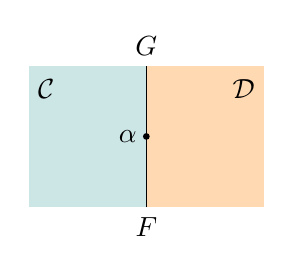
\begin{tikzpicture}
\def\x{0};
\def\xl{-1.5};
\def\xr{1.5};


\def \ya{0.8};
\def \yb{1.7};
\def \yc{2.6};
\def \yt {2.3};

\filldraw[fill=blue!50!green!20, draw=white] (\xl, \ya) rectangle (\x, \yc);
\filldraw[fill=orange!30, draw=white] (\x, \ya) rectangle (\xr, \yc);

\node[below] (a) at (\x, \ya) {$F$};
\node(b) at (\x, \yb) {};
\node [above] (c) at (\x, \yc) {$G$};

\node(l)[right] at (\xl, \yt) {$\mathcal{C}$};
\node(r)[left] at (\xr, \yt) {$\mathcal{D}$};


\filldraw[black] (b) circle (1 pt);
\node [left] at (b) {$\alpha$};

\draw (a)  -- (c);

\end{tikzpicture}
\]

This is an example of a \emph{string diagram}. You read such a digram bottom-up, left-to-right (think of the $(x, y)$ system of coordinates). 

The bottom of this diagram shows a functor $F$ that goes from $\mathcal{C}$ to $\mathcal{D}$. The top of the diagram shows a functor $G$ that goes between the same two categories. The transition happens in the middle, where a natural transformation $\alpha$ maps $F$ to $G$.

So far, it doesn't seem like we gain a lot by using this new visual representation. But let's apply it to something more interesting: vertical composition of natural transformations:
\[
\begin{tikzcd}[column sep=huge]
\mathcal{C}
  \arrow[bend left=60]{rr}[name=U, label=above:$H$]{}
  \arrow[]{rr}[name=M, label={[xshift=15pt, yshift=-5pt]:$G$}]{} 
  \arrow[bend right=60]{rr}[name=D, label=below:$F$]{} 
 &&
\mathcal{D}
  \arrow[shorten <=8pt, shorten >=8pt,Leftarrow, to path={(U) -- node[label=left:$\beta$] {} (M)}]{}
  \arrow[shorten <=8pt, shorten >=8pt,Leftarrow, to path={(M) -- node[label=left:$\alpha$] {} (D)}]{}
\end{tikzcd}
\]

The corresponding string diagram shows the two categories and three functors between them joined by two natural transformations.
\[
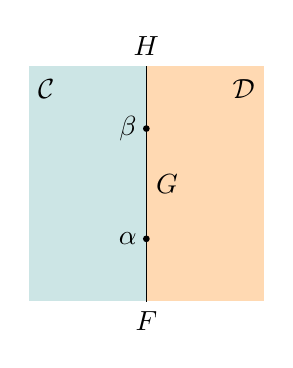
\begin{tikzpicture}
\def\x{0};
\def\xl{-1.5};
\def\xr{1.5};


\def \ya{0};
\def \yb{0.8};
\def \ybb{2.2};
\def \yc{3};
\def \yt {2.7};
\def \ymid {1.5}

\filldraw[fill=blue!50!green!20, draw=white] (\xl, \ya) rectangle (\x, \yc);
\filldraw[fill=orange!30, draw=white] (\x, \ya) rectangle (\xr, \yc);

\node[below] (a) at (\x, \ya) {$F$};
\node(b) at (\x, \yb) {};
\node(bb) at (\x, \ybb) {};
\node [above] (c) at (\x, \yc) {$H$};
\node(m)[right] at (\x, \ymid) {$G$};

\node(l)[right] at (\xl, \yt) {$\mathcal{C}$};
\node(r)[left] at (\xr, \yt) {$\mathcal{D}$};

\filldraw[black] (b) circle (1 pt);
\node [left] at (b) {$\alpha$};
\filldraw[black] (bb) circle (1 pt);
\node [left] at (bb) {$\beta$};

\draw (a)  -- (c);

\end{tikzpicture}
\]
As you can see, you can reconstruct the original diagram from the string diagram by scanning it bottom-to-top.

Let's continue with the horizontal composition of natural transformations:
\[
\begin{tikzcd}[column sep=huge]
\mathcal{C}
  \arrow[bend left=50]{r}[name=U, label=above:$F'$]{}
  \arrow[bend right=50]{r}[name=D, label=below:$F$]{} 
 &
\mathcal{D}
  \arrow[bend left=50]{r}[name=U1, label=above:$G'$]{}
  \arrow[bend right=50]{r}[name=D1, label=below:$G$]{} 
 &
\mathcal{E}
  \arrow[shorten <=10pt,shorten >=10pt,Leftarrow,to path={(U) -- node[label=left:$\alpha$] {} (D)}]{}
  \arrow[shorten <=10pt,shorten >=10pt,Leftarrow,to path={(U1) -- node[label=left:$\beta$] {} (D1)}]{}
\end{tikzcd}
\]
This time we have three categories, so we'll have three areas. 

The bottom of the string diagram corresponds to the composition of functors $G \circ F$ (in this order). The top corresponds to $G' \circ F'$. One natural transformation, $\alpha$, connects $F$ to $F'$; the other, $\beta$, connects $G$ to $G'$.
\[
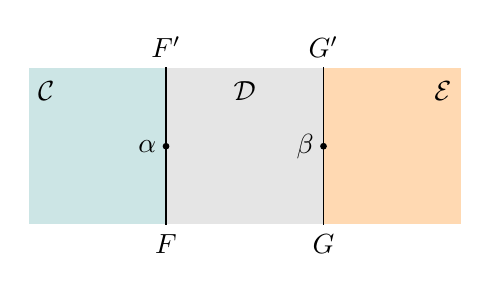
\begin{tikzpicture}
\def\xl{-2.75};
\def\xa{-1};
\def\xc{0}
\def\xb{1};
\def\xr{2.75};


\def \ya{0};
\def \yb{1};
\def \yc{2};
\def \yt {1.7};

\filldraw[fill=blue!50!green!20, draw=white] (\xl, \ya) rectangle (\xa, \yc);
\filldraw[fill=black!10!white, draw=white] (\xa, \ya) rectangle (\xb, \yc);
\filldraw[fill=orange!30, draw=white] (\xb, \ya) rectangle (\xr, \yc);

\node[below] (a) at (\xa, \ya) {$F$};
\node(b) at (\xa, \yb) {};
\node [above] (c) at (\xa, \yc) {$F'$};

\node[below] (d) at (\xb, \ya) {$G$};
\node(e) at (\xb, \yb) {};
\node [above] (f) at (\xb, \yc) {$G'$};

\node(l)[right] at (\xl, \yt) {$\mathcal{C}$};
\node(r) at (\xc, \yt) {$\mathcal{D}$};
\node(r)[left] at (\xr, \yt) {$\mathcal{E}$};


\filldraw[black] (b) circle (1 pt);
\node [left] at (b) {$\alpha$};
\filldraw[black] (e) circle (1 pt);
\node [left] at (e) {$\beta$};

\draw (a)  -- (c);
\draw (d)  -- (f);

\end{tikzpicture}
\]
Drawing two parallel vertical lines, in this new system, corresponds to functor composition. You can think of the composition of natural transformations as happening along the imaginary horizontal line in the middle of the diagram. But what if somebody was sloppy in drawing the diagram, and one of the dots was a little higher than the other? As it turns out, the exact positioning of the dots doesn't matter, due to the interchange law.

But first, let's illustrate whiskering: horizontal composition in which one of the natural transformation is the identity. We can draw it like this:

\[
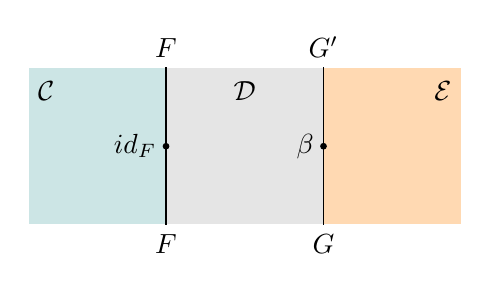
\begin{tikzpicture}
\def\xl{-2.75};
\def\xa{-1};
\def\xc{0}
\def\xb{1};
\def\xr{2.75};


\def \ya{0};
\def \yb{1};
\def \yc{2};
\def \yt {1.7};

\filldraw[fill=blue!50!green!20, draw=white] (\xl, \ya) rectangle (\xa, \yc);
\filldraw[fill=black!10!white, draw=white] (\xa, \ya) rectangle (\xb, \yc);
\filldraw[fill=orange!30, draw=white] (\xb, \ya) rectangle (\xr, \yc);

\node[below] (a) at (\xa, \ya) {$F$};
\node(b) at (\xa, \yb) {};
\node [above] (c) at (\xa, \yc) {$F$};

\node[below] (d) at (\xb, \ya) {$G$};
\node(e) at (\xb, \yb) {};
\node [above] (f) at (\xb, \yc) {$G'$};

\node(l)[right] at (\xl, \yt) {$\mathcal{C}$};
\node(r) at (\xc, \yt) {$\mathcal{D}$};
\node(r)[left] at (\xr, \yt) {$\mathcal{E}$};


\filldraw[black] (b) circle (1 pt);
\node [left] at (b) {$id_F$};
\filldraw[black] (e) circle (1 pt);
\node [left] at (e) {$\beta$};

\draw (a)  -- (c);
\draw (d)  -- (f);

\end{tikzpicture}
\]
But, really, the identity can be inserted at any point on a vertical line, so we don't even have to draw it. The following diagram represents the whiskering of $\beta \circ F$.
\[
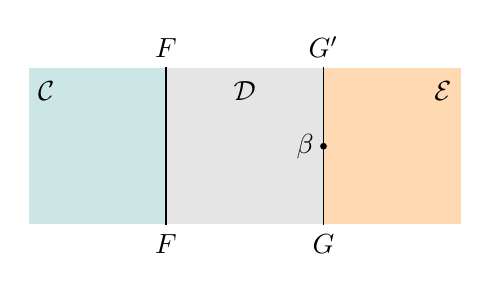
\begin{tikzpicture}
\def\xl{-2.75};
\def\xa{-1};
\def\xc{0}
\def\xb{1};
\def\xr{2.75};


\def \ya{0};
\def \yb{1};
\def \yc{2};
\def \yt {1.7};

\filldraw[fill=blue!50!green!20, draw=white] (\xl, \ya) rectangle (\xa, \yc);
\filldraw[fill=black!10!white, draw=white] (\xa, \ya) rectangle (\xb, \yc);
\filldraw[fill=orange!30, draw=white] (\xb, \ya) rectangle (\xr, \yc);

\node[below] (a) at (\xa, \ya) {$F$};
\node(b) at (\xa, \yb) {};
\node [above] (c) at (\xa, \yc) {$F$};

\node[below] (d) at (\xb, \ya) {$G$};
\node(e) at (\xb, \yb) {};
\node [above] (f) at (\xb, \yc) {$G'$};

\node(l)[right] at (\xl, \yt) {$\mathcal{C}$};
\node(r) at (\xc, \yt) {$\mathcal{D}$};
\node(r)[left] at (\xr, \yt) {$\mathcal{E}$};

\filldraw[black] (e) circle (1 pt);
\node [left] at (e) {$\beta$};

\draw (a)  -- (c);
\draw (d)  -- (f);

\end{tikzpicture}
\]
You can easily imagine the diagram for $\alpha \circ G$.

Here's the string diagram that corresponds to the interchange law:
\[
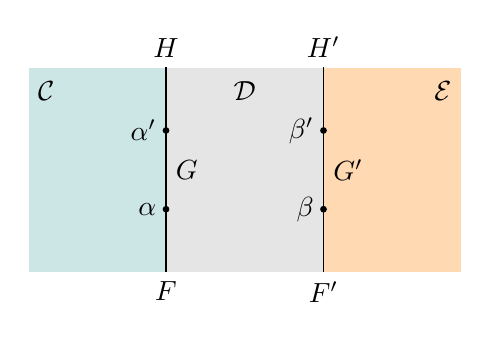
\begin{tikzpicture}
\def\xl{-2.75};
\def\xa{-1};
\def\xc{0}
\def\xb{1};
\def\xr{2.75};


\def \ya{0.2};
\def \yb{1};
\def \ybb{2}
\def \yc{2.8};
\def \yt {\yc -0.3};
\def \ymid {1.5}

\filldraw[fill=blue!50!green!20, draw=white] (\xl, \ya) rectangle (\xa, \yc);
\filldraw[fill=black!10!white, draw=white] (\xa, \ya) rectangle (\xb, \yc);
\filldraw[fill=orange!30, draw=white] (\xb, \ya) rectangle (\xr, \yc);

\node[below] (a) at (\xa, \ya) {$F$};
\node(b) at (\xa, \yb) {};
\node [above] (c) at (\xa, \yc) {$H$};
\node [right] (ml) at (\xa, \ymid) {$G$};

\node[below] (d) at (\xb, \ya) {$F'$};
\node(e) at (\xb, \yb) {};
\node [above] (f) at (\xb, \yc) {$H'$};
\node [right] (ml) at (\xb, \ymid) {$G'$};

\node(l)[right] at (\xl, \yt) {$\mathcal{C}$};
\node(r) at (\xc, \yt) {$\mathcal{D}$};
\node(r)[left] at (\xr, \yt) {$\mathcal{E}$};


\filldraw[black] (b) circle (1 pt);
\node [left] at (b) {$\alpha$};
\filldraw[black] (e) circle (1 pt);
\node [left] at (e) {$\beta$};

\node(bb) at (\xa, \ybb) {};
\node(ee) at (\xb, \ybb) {};

\filldraw[black] (bb) circle (1 pt);
\node [left] at (bb) {$\alpha'$};
\filldraw[black] (ee) circle (1 pt);
\node [left] at (ee) {$\beta'$};

\draw (a)  -- (c);
\draw (d)  -- (f);

\end{tikzpicture}
\]
This diagram is purposefully ambiguous. Are we supposed to first do vertical composition of natural transformations and then the horizontal one? Or should we compose $\beta \circ \alpha$ and $\beta' \circ \alpha'$ horizontally, and then compose the results vertically? The interchange law says that it doesn't matter: the result is the same. 

Now try to replace a pair of natural transformations in this diagram with identities. If you replace $\alpha'$ and $\beta'$, you get the horizontal composition of $\beta \circ \alpha$. If you replace $\alpha'$ and $\beta$, and rename $\beta'$ to $\beta$, you get the diagram in which $\alpha$ is shifted down with respect to $\beta$, and so on. The interchange law tells us that all these diagrams are equal. We are free to slide natural transformations like beads on a string.

\subsection{String diagrams for the monad}

A monad is defined as an endofunctor and two natural transformations illustrated by the following diagrams:
 
\[
\begin{tikzcd}[column sep=huge]
\mathcal{C}
  \arrow[bend left=50]{r}[name=U, label=above:$T$]{}
  \arrow[bend right=50]{r}[name=D, label=below:$\text{Id}$]{} 
 &
\mathcal{C}
  \arrow[shorten <=10pt,shorten >=10pt,Leftarrow,to path={(U) -- node[label=left:$\eta$] {} (D)}]{}
\end{tikzcd}
\hspace{20pt}
\begin{tikzcd}[column sep=huge]
\mathcal{C}
  \arrow[bend left=50]{r}[name=U, label=above:$T$]{}
  \arrow[bend right=50]{r}[name=D, label=below:$T \circ T$]{} 
 &
\mathcal{C}
  \arrow[shorten <=10pt,shorten >=10pt,Leftarrow,to path={(U) -- node[label=left:$\mu$] {} (D)}]{}
\end{tikzcd}
\]

Since we are dealing with just one category, when translating these diagrams to string diagrams, we can dispose of the naming (and shading) of categories, and just draw the strings alone.
\[
\begin{tikzpicture}

\def \xleft{-2}

\def\xa{0};
\def\xb{0.7};
\def\xc{\xb * 2};

\def \ya{0};
\def \yb{1};
\def \yc{2};

\node(a) at (\xleft, \ya) {};
\node(b) at (\xleft, \yb) {}; % middle
\node(c) at (\xleft, \yc) {};

\draw[dashed] (a) -- node[right] {$\text{Id}$} (b);
\draw (b) -- node[right] {$T$} (c);


\node(d) at (\xa, \ya) {};
\node(e) at (\xc, \ya) {};
\node(f) at (\xb, \yb) {}; % middle
\node(g) at (\xb, \yc) {}; % top


\filldraw[black] (b) circle (1 pt);
\node [left] at (b) {$\eta$};

\draw (d) to [out=90, in=180]  node[left] {$T$}(f);
\draw (e) to [out=90, in=0]  node[right] {$T$} (f);

\draw (f) -- node[right] {$T$} (g);

\filldraw[black] (f) circle (1 pt);
\node [below] at (f) {$\mu$};

\end{tikzpicture}
\]
In the first diagram, it's customary to skip the dashed line corresponding to the identity functor. The $\eta$ dot can freely inject a $T$ line into a diagram. Two $T$ lines can be joined by the $\mu$ dot. 

String diagrams are especially useful in expressing monad laws. For instance, we have the left identity law:
\[ \mu \circ (\eta \circ T) = id \]
which can be visualized as a commuting diagram:
\[
 \begin{tikzcd}
 \text{Id} \circ T
 \arrow[rr, "\eta \circ T"]
 \arrow[rrd, "id"']
& & T \circ T
 \arrow[d, "\mu"]
 \\
 && T
  \end{tikzcd}
\]
The corresponding string diagram is a pictorial representation of the equality of the two paths through this diagram:
\[
\begin{tikzpicture}
\def\xa{0};
\def\xb{0.7};
\def\xc{\xb * 2};

\def \ya{0.8};
\def \yb{1.7};
\def \yc{2.6};

\node(a) at (\xa, \ya) {};
\node(b) at (\xb, \yb) {};
\node(c) at (\xc, 0) {};
\node(d) at (\xb, \yc) {};
\filldraw[black] (a) circle (1 pt);
\node [below] at (a) {$\eta$};
\filldraw[black] (b) circle (1 pt);
\node [below] at (b) {$\mu$};
\draw (a) to [out=90, in=180]  node[left] {$T$}(b);
\draw (c) to [out=90, in=0]  node[right] {$T$} (b);
\draw (b) -- node[right] {$T$} (d);

\def\xd{3.5}
\def\xe{2.5}
\node(e) at (\xd, 0) {};
\node(f) at (\xd, \yc) {};
\node at (\xe, 1.5) {$=$};
\draw (e) -- node[right] {$T$} (f);
\end{tikzpicture}
\]
You can think of this equality as the result of pulling on the top and bottom strings resulting in the $\eta$ appendage being retracted into the straight line.

There is a symmetric right identity law:
\[
\begin{tikzpicture}
\def\xa{0};
\def\xb{0.7};
\def\xc{\xb * 2};

\def \ya{0.8};
\def \yb{1.7};
\def \yc{2.6};

\node(a) at (\xa, 0) {};
\node(b) at (\xb, \yb) {};
\node(c) at (\xc, \ya) {};
\node(d) at (\xb, \yc) {};
\filldraw[black] (b) circle (1 pt);
\node [below] at (c) {$\eta$};
\filldraw[black] (c) circle (1 pt);
\node [below] at (b) {$\mu$};
\draw (a) to [out=90, in=180]  node[left] {$T$}(b);
\draw (c) to [out=90, in=0]  node[right] {$T$} (b);
\draw (b) -- node[right] {$T$} (d);

\def\xd{3.5}
\def\xe{2.5}
\node(e) at (\xd, 0) {};
\node(f) at (\xd, \yc) {};
\node at (\xe, 1.5) {$=$};
\draw (e) -- node[right] {$T$} (f);
\end{tikzpicture}
\]

Finally, this is the associativity law in terms of string diagrams:
\[
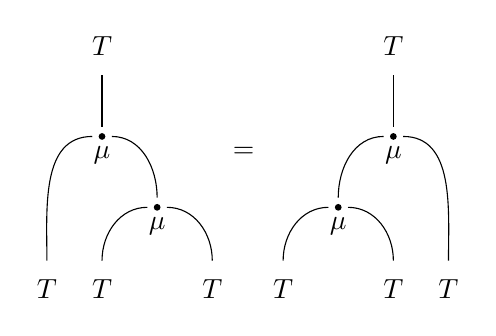
\begin{tikzpicture}
\def\delta{0.7}
\def\xa{0};
\def\xb{\delta};
\def\xc{\delta * 2};
\def\xd{\delta * 3};

\def \ya{0.8};
\def \yb{1.7};
\def \yc{2.6};

\node(a) at (\xa, 0) {};
\node(b) at (\xb, \yb) {};
\node(c) at (\xc, \ya) {};
\node(d) at (\xb, \yc) {};
\node(e) at (\xb, 0) {};
\node(f) at (\xd, 0) {};
\filldraw[black] (b) circle (1 pt);
\filldraw[black] (c) circle (1 pt);
\node [below] at (b) {$\mu$};
\draw (a) to [out=90, in=180]  node[left] {}(b);
\draw (c) to [out=90, in=0]  node[right] {} (b);
\draw (b) -- node[right] {} (d);
\draw (e) to [out=90, in=180]  node[left] {}(c);
\draw (f) to [out=90, in=0]  node[right] {}(c);
\node [below] at (c) {$\mu$};
\node [below] at (a) {$T$};
\node [above] at (d) {$T$};
\node [below] at (e) {$T$};
\node [below] at (f) {$T$};

\def\xe{2.5}
\node at (\xe, 1.5) {$=$};

\def\off{3}
\def\xa{\off + \delta * 0};
\def\xb{\off + \delta * 1};
\def\xc{\off + \delta * 2};
\def\xd{\off + \delta * 3};

\node(a) at (\xa, 0) {};
\node(b) at (\xc, 0) {};
\node(c) at (\xd, 0) {};
\node(d) at (\xb, \ya) {};
\node(e) at (\xc, \yb) {};
\node(f) at (\xc, \yc) {};
\filldraw[black] (d) circle (1 pt);
\filldraw[black] (e) circle (1 pt);
\node [below] at (d) {$\mu$};
\draw (a) to [out=90, in=180]  node[left] {}(d);
\draw (b) to [out=90, in=0]  node[right] {} (d);
\draw (e) -- node[right] {} (f);
\draw (d) to [out=90, in=180]  node[left] {}(e);
\draw (c) to [out=90, in=0]  node[right] {}(e);
\node [below] at (e) {$\mu$};
\node [below] at (a) {$T$};
\node [below] at (b) {$T$};
\node [below] at (c) {$T$};
\node [above] at (f) {$T$};
\end{tikzpicture}
\]

\subsection{String diagrams for the adjunction}

An adjunction is a relation between a pair of functors, $L \colon \mathcal{D} \to \mathcal{C}$ and $R \colon \mathcal{C} \to \mathcal{D}$. It can be defined by a pair of natural transformations, the unit $\eta$ and the counit $\varepsilon$, satisfying triangular identities.

The unit of the adjunction can be illustrated by a ``cup''-shaped diagram:

\[
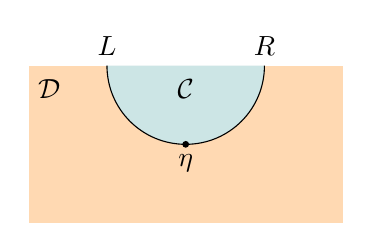
\begin{tikzpicture}

\def \xrightmost {2}
\def \xright         {1}
\def \xmid          {0}
\def \xleft           {-\xright}
\def \xleftmost   {-\xrightmost}

\def \ybot           {0}
\def \ymid          {1}
\def \ytop           {2}
\def \ylabel        {\ytop - 0.3}

% functor labels
\node [above] at (\xleft, \ytop)   {$L$};
\node [above] at (\xright, \ytop) {$R$};
% background
\filldraw[fill=orange!30, draw=white] (\xleftmost, \ytop) rectangle (\xrightmost, \ybot);
% cup
\draw [fill=blue!50!green!20] (\xleft, \ytop) to [out=-90, in=180] (\xmid, \ymid) to [out=0, in=-90] (\xright, \ytop);
% natural transformation
\filldraw [black] (\xmid, \ymid) circle (1 pt);
\node [below] at (\xmid, \ymid) {$\eta$};
% category labels
\node           at (\xmid, \ylabel)        {$\mathcal{C}$};
\node [right] at (\xleftmost, \ylabel) {$\mathcal{D}$};

\end{tikzpicture}
\]
The identity functor at the bottom of the diagram is omitted from the picture. The $\eta$ dot turns the identity functor below it to the composition $R \circ L$ above it.

Similarly, the counit can be visualized as a ``cap''-shaped string diagram with the implicit identity functor at the top:

\[
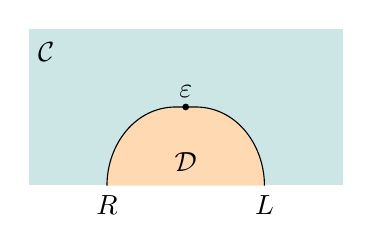
\begin{tikzpicture}
\def\xleft{0};
\def\xmid{1};
\def\xright{\xmid * 2};

\def \ybot{0};
\def \ymid{1};
\def \ytop{2 * \ymid};
\def \yt{2 * \ymid - 0.3};

\node [below] (a) at (\xleft, \ybot) {$R$};
\node(b) at (\xmid, \ymid) {};
\node[below] (c) at (\xright, \ybot) {$L$};

\filldraw[fill=blue!50!green!20, draw=white] (\xleft-1, \ytop) rectangle (\xright+1, \ybot);


\draw [fill=orange!30] (a.north) to [out=90, in=180] (b.west) -- (b.east) to [out=0, in=90] (c.north);

\filldraw[black] (b) circle (1 pt);
\node [above] at (b) {$\varepsilon$};

\node(l)[right] at (\xleft-1, \yt) {$\mathcal{C}$};
\node(r) at (\xmid, \ybot + 0.3) {$\mathcal{D}$};

\end{tikzpicture}
\]

Triangle identities can be easily expressed using string diagrams. They also make intuitive sense, as you can imagine pulling on the string from both sides to straighten the curve.

For instance, this is the first triangle identity. 

\[
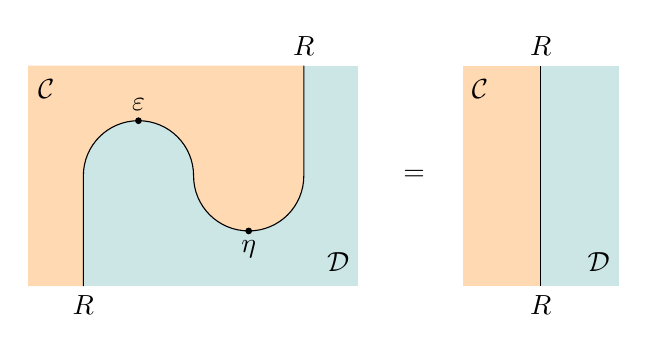
\begin{tikzpicture}
\def \dx {0.7}
\def \dy {0.7}

\def \xa{-3 * \dx};
\def \xb{-2 * \dx};
\def \xc{-1 * \dx};
\def \xd{0};
\def \xe{1 * \dx};
\def \xf{2 * \dx};
\def \xg{3 * \dx};

\def \ya{0};
\def \yb{1 * \dy};
\def \yc{2 * \dy};
\def \yd{3 * \dy};
\def \ye{4 * \dy};

\node [below] at (\xb, \ya) {$R$};
\node [right] at (\xd, \yc) {$L$};
\node [above] at (\xf, \ye) {$R$};
% background
\filldraw[fill=blue!50!green!20, draw=white] (\xa, \ye) rectangle (\xg, \ya);
% fill shape
\path [fill=orange!30] (\xa, \ya) to (\xb, \ya) to (\xb, \yc) to [out=90, in=180]  (\xc, \yd) to  [out=0, in=90] (\xd, \yc) to [out=-90, in=180] (\xe, \yb) to [out=0, in=-90] (\xf, \yc) to (\xf, \ye) to (\xa, \ye);

\draw (\xb, \ya) to (\xb, \yc) to [out=90, in=180]  (\xc, \yd) to  [out=0, in=90] (\xd, \yc) to [out=-90, in=180] (\xe, \yb) to [out=0, in=-90] (\xf, \yc) to (\xf, \ye);

\filldraw[black] (\xc, \yd) circle (1 pt);
\node [above] at (\xc, \yd) {$\varepsilon$};

\filldraw[black] (\xe, \yb) circle (1 pt);
\node [below] at (\xe, \yb) {$\eta$};

\node[right] at (\xa, \ye - 0.3) {$\mathcal{C}$};
\node[left] at (\xg, \ya + 0.3) {$\mathcal{D}$};

% right diagram

\node (eq) at (4 * \dy, \yc) {$=$};
\def \xh {6.3 * \dx}

\filldraw[fill=orange!30, draw=white] (\xh - 1, \ye) rectangle (\xh, \ya);
\filldraw[fill=blue!50!green!20, draw=white] (\xh, \ye) rectangle (\xh + 1, \ya);

\draw (\xh, \ye) -- (\xh, \ya);

\node[below] (bb) at (\xh, \ya) { $R$ };
\node[above] (bt) at (\xh, \ye) { $R$ };

\node(l)[right] at (\xh - 1, \ye - 0.3) {$\mathcal{C}$};
\node(r)[left] at (\xh + 1, \ya + 0.3) {$\mathcal{D}$};

\end{tikzpicture}
\]
Reading the left diagram bottom-to-top produces a series of mappings:

\[  Id_{\mathcal{D}} \circ R \xrightarrow{\eta \circ R} R \circ L \circ R \xrightarrow{R \circ \varepsilon} R \circ Id_{\mathcal{C}}  \]
This is supposed to be equal to the right-hand-side, which is the identity natural transformation on $R$

\begin{exercise}
Draw the string diagrams for the second triangle identity.
\end{exercise}

\section{Monads from Adjunctions}

You might have noticed that the same symbol $\eta$ is used for the unit of the adjunction and for the unit of the monad. This is \emph{not} a coincidence. 

At first sight it might seem like comparing apples to oranges: an adjunction is defined using two functors between two categories and a monad is defined by one endofunctor operating on a single category. However, the composition of the two functors is an endofunctor and the unit of the adjunction maps the identity functor to this composite $R \circ L$. 

Compare this diagram
\[
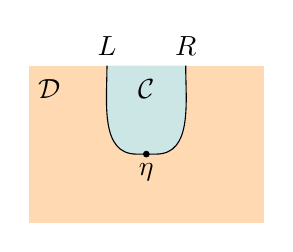
\begin{tikzpicture}
\def\xleft{0.5};
\def\xmid{1};
\def\xright{1.5};

\def \ybot{0};
\def \ymid{1};
\def \ytop{2 * \ymid};
\def \yt{2 * \ymid - 0.3};

\node [above] (a) at (\xleft, \ytop) {$L$};
\node(b) [below] at (\xmid, \ymid) {};
\node[above] (c) at (\xright, \ytop) {$R$};

\filldraw[fill=orange!30, draw=white] (\xleft-1, \ytop) rectangle (\xright+1, \ybot);


\draw [fill=blue!50!green!20] (a.south) to [out=-90, in=180] (b.west) -- (b.east) to [out=0, in=-90] (c.south);
\filldraw[black] (b) circle (1 pt);
\node [below] at (b) {$\eta$};

\node(l)[right] at (\xleft-1, \yt) {$\mathcal{D}$};
\node(r) at (\xmid, \yt) {$\mathcal{C}$};

\end{tikzpicture}
\]
with the one defining the monadic unit:

\[
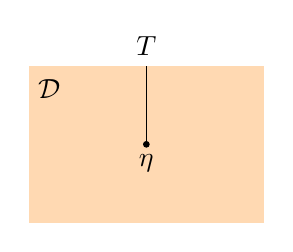
\begin{tikzpicture}
\def\xleft{0.5};
\def\xmid{1};
\def\xright{1.5};

\def \ybot{0};
\def \ymid{1};
\def \ytop{2 * \ymid};
\def \yt{2 * \ymid - 0.3};

\node(b) [above] at (\xmid, \ytop) {$T$};

\filldraw[fill=orange!30, draw=white] (\xleft-1, \ytop) rectangle (\xright+1, \ybot);

\draw (\xmid, \ymid) -- (\xmid, \ytop);

\filldraw[black] (\xmid, \ymid) circle (1 pt);
\node [below] at (\xmid, \ymid) {$\eta$};

\node(l)[right] at (\xleft-1, \yt) {$\mathcal{D}$};

\end{tikzpicture}
\]
It turns out that $T = R \circ L$ is in fact a monad, with the multiplication $\mu$ defined by the following diagram:

\[
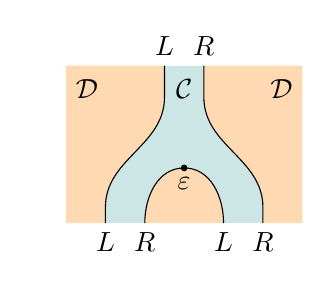
\begin{tikzpicture}
\def \xmid          {0};
\def \xr               {0.5};
\def \xrr             {1}
\def \xrm            {0.25}
\def \xrightmost {1.5}
\def \xl {-\xr}
\def \xll {-\xrr}
\def \xlm {-\xrm}
\def \xleftmost {-\xrightmost}

\def \ybot           {0};
\def \ymidbot     {0.20};
\def \yeps          {0.7};
\def \ymid          {1};
\def \ymidtop     {1.60}
\def \ytop           {2};
\def \ylabel        {\ytop - 0.3};
% functors
\node [above] at (\xlm, \ytop)  {$L$};
\node [above] at (\xrm, \ytop) {$R$};
\node [below] at (\xll, \ybot) {$L$};
\node [below] at (\xl, \ybot) {$R$};
\node [below] at (\xr, \ybot) {$L$};
\node [below] at (\xrr, \ybot) {$R$};

\filldraw[fill=blue!50!green!20, draw=white, draw=white] (\xleftmost, \ytop) rectangle (\xrightmost, \ybot);

% left area
\path [fill=orange!30] (\xleftmost, \ybot) to  (\xll, \ybot) to (\xll, \ymidbot) [out=90, in=-90] to (\xlm, \ymidtop) to  (\xlm, \ytop) to [out=180, in=180] (\xleftmost, \ytop);
% right area
\path [fill=orange!30] (\xrightmost, \ybot) to (\xrr, \ybot) to (\xrr, \ymidbot) [out=90, in=-90] to (\xrm, \ymidtop) to (\xrm, \ytop) to [out=0, in=180]  (\xrightmost, \ytop);
% cap
\draw [fill=orange!30] (\xl, \ybot) to [out=90, in=180] (\xmid, \yeps) to [out=0, in=90] (\xr, \ybot);
% left curve
\draw (\xll, \ybot) to (\xll, \ymidbot) [out=90, in=-90] to (\xlm, \ymidtop) to  (\xlm, \ytop);
% right curve
\draw (\xrr, \ybot) to (\xrr, \ymidbot) [out=90, in=-90] to (\xrm, \ymidtop) to (\xrm, \ytop);
% epsilon
\filldraw [black] (\xmid, \yeps) circle (1 pt);
\node [below] at (\xmid, \yeps) {$\varepsilon$};
% categories
\node [right] at (\xleftmost, \ylabel) {$\mathcal{D}$};
\node           at (\xmid, \ylabel)        {$\mathcal{C}$};
\node [left]   at (\xrightmost, \ylabel) {$\mathcal{D}$};

\end{tikzpicture}
\]
Reading this diagram bottom-up, we get the following transformation (imagine slicing it horizontally at the dot):
\[  R \circ L \circ R \circ L \xrightarrow{R \circ \varepsilon \circ L} R \circ L  \]
Compare this with the definition of monadic $\mu$:

\[
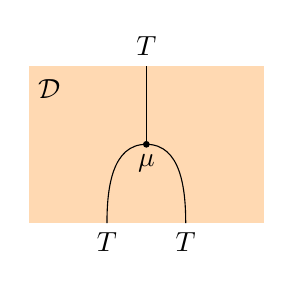
\begin{tikzpicture}
\def \xmid          {0};
\def \xr               {0.5};
\def \xrightmost {1.5};
\def \xl {-\xr};
\def \xleftmost {-\xrightmost};

\def \ybot           {0};
\def \ymid          {1};
\def \ytop           {2};
\def \ylabel        {\ytop - 0.3};

\node [above] at (\xmid, \ytop) {$T$};
\node [below] at (\xl, \ybot)      {$T$};
\node [below] at (\xr, \ybot)      {$T$};

\filldraw[fill=orange!30, draw=white] (\xleftmost, \ytop) rectangle (\xrightmost, \ybot);
% cap
\draw (\xl, \ybot) to [out=90, in=180] (\xmid, \ymid) to [out=0, in=90] (\xr, \ybot);
\draw (\xmid, \ymid) to (\xmid, \ytop);

\filldraw [black] (\xmid, \ymid) circle (1 pt);
\node [below] at (\xmid, \ymid) {$\mu$};

\node [right] at (\xleftmost, \ylabel) {$\mathcal{D}$};

\end{tikzpicture}
\]
This gives us the definition of $\mu$ for the monad $R \circ L$ as the double-whiskering of $\varepsilon$:
\[ \mu = R \circ \varepsilon \circ L \]

To complete the picture, we can use string diagrams to derive monadic laws using triangle identities. The trick is to replace all strings in monadic laws by pairs of parallel strings and then rearrange them according to the rules.

To summarize, every adjunction $L \dashv R$ with the unit $\eta$ and counit $\varepsilon$ defines a monad $(R \circ L, \eta, R \circ \varepsilon \circ L)$.

In the next chapter we'll see that, dually, the other composition, $L \circ R$ defines a comonad.

\begin{exercise}
Draw string diagrams to illustrate monadic laws (unit and associativity) for the monad derived from an adjunction.
\end{exercise}

\section{Examples of Monads from Adjunctions}

We'll go through several examples of adjunctions that generate the monads that we use in programming. Most examples involve functors that leave the category of Haskell types and functions, even though the round trip that generates the monad is an endofunctor. This is why it's often impossible to express the adjunction in Haskell. 

To additionally complicate things, there is a lot of bookkeeping related to explicit naming of data constructors, which is necessary for type inference to work. This may sometimes obscure the simplicity on the underlying formulas.

\subsection{Free monoid and the list monad}
The list monad corresponds to the free monoid adjunction. The unit of this adjunction, $\eta_X \colon X \to U (F X)$, injects the elements of the set $X$ as the generators of the free monoid. We represent the free monoid as a list, and its generators are singleton lists. Compare this with the monadic unit:
\begin{haskell}
return x = [x]
\end{haskell}
To implement the counit of this adjunction, $\varepsilon_M \colon F (U M) \to M$, we take a monoid $M$, forget its multiplication, and use its sets of elements as generators for the free monoid. The counit is a monoid morphism from that free monoid back to $M$, which is a special case of a catamorphism. Recall the Haskell implementation of a list catamorphism:
\begin{haskell}
foldMap :: Monoid m => (a -> m) -> ([a] -> m)
foldMap f = foldr mappend mempty . fmap f
\end{haskell}
The counit is just \hask{foldMap id}, or 
\begin{haskell}
epsilon = foldr mappend mempty
\end{haskell}
Monad multiplication is given by the whiskering of the counit:
\[ \mu = U \circ \varepsilon \circ F \]
You can easily convince yourself that left whiskering doesn't do much here, since it's just a lifting of a monoid morphism by the forgetful functor. It just keeps the function, forgetting about it's special property of preserving structure. The right whiskering by $F$ is more interesting. It means taking the component of $\varepsilon$ at a free monoid generated from the set $X$. For this monoid we have 
\begin{haskell}
mempty = []
mappend = (++)
\end{haskell}
Thich gives us the definition of $\mu$ or \hask{join}:
\begin{haskell}
join = foldr (++) []
\end{haskell}
which is the same as \hask{concat}.

\subsection{The currying adjunction and the state monad}

The state monad is generated by the adjunction between two endofunctors that define the exponential object. The left functor is defined by a product with some fixed object $S$:
\[ L_S A = A \times S \]
We can implement it as a Haskell type:
\begin{haskell}
newtype L s a = L (a, s)
\end{haskell}
The right functor produces the exponential object, parameterized by the same object $S$:
\[ R_S C = C^S \]
In Haskell, it's a thinly encapsulated function type:
\begin{haskell}
newtype R s c = R (s -> c)
\end{haskell}

The monad is given by the composition of these two functors:
\[(R_S \circ L_S) A = (A \times S)^S \]
In Haskell we would write it as:
\begin{haskell}
newtype St s a = St (R s (L s a))
\end{haskell}
If you expand this definition, it's easy to recognize in it the \hask{State} functor:
\begin{haskell}
newtype State s a = State (s -> (a, s))
\end{haskell}

The unit of the adjunction $L_S \dashv R_S$ is:
\[ \eta_A \colon A \to (A \times S)^S \]
which can be implemented in Haskell as:
\begin{haskell}
eta :: a -> R s (L s a)
eta a = R (\s -> L (a, s))
\end{haskell}
You may recognized in it a thinly veiled version of \hask{return} for the state monad:
\begin{haskell}
return :: a -> State s a
return a = State (\s -> (a, s))
\end{haskell}

Here's the component of the counit of this adjunction at $C$:
\[ \varepsilon_C \colon C^S \times S \to C \]
It can be implemented in Haskell as:
\begin{haskell}
epsilon :: L s (R s a) -> a
epsilon (L ((R f), s))= f s
\end{haskell}
which, after stripping data constructors, is equivalent to \hask{apply}, or the uncurried version of \hask{runState}.

Monad multiplication $\mu$ is given by whiskering $\varepsilon$ from both sides:
\[ \mu = R_S \circ \varepsilon \circ L_S \]
This is how it translates to Haskell:
\begin{haskell}
mu :: R s (L s (R s (L s a))) -> R s (L s a)
mu = fmap epsilon
\end{haskell}
Here, whiskering on the right doesn't do anything other than select a component of the natural transformation. This is done automatically by Haskell's type inference engine. Whiskering on the left is done by lifting the component of the natural transformation. Again, type inference picks the correct implementation of \hask{fmap} (here, it's equivalent to precomposition) to perform that.

Compare this with the implementation of \hask{join}:
\begin{haskell}
join :: State s (State s a) -> State s a
join mma = State (fmap (uncurry runState) (runState mma))
\end{haskell}
Notice the dual use of \hask{runState}: 
\begin{haskell}
runState :: State s a -> s -> (a, s)
runState (State h) s = h s
\end{haskell}
When it's uncurried, its type signature becomes:
\begin{haskell}
uncurry runState :: (State s a , s) -> (a, s)
\end{haskell}
which is equivalent to that of \hask{epsilon}. When partially applied, it just strips the data constructor exposing the underlying function type:
\begin{haskell}
runState st ::  s -> (a, s)
\end{haskell}



\subsection{M-sets and the writer monad}

The writer monad:
\begin{haskell}
newtype Writer m a = Writer (a, m)
\end{haskell}
is parameterized by a monoid \hask{m}. This monoid is used for accumulating log entries. The adjunction we are going to use involves a category of M-sets for that monoid. 

An M-set is a set $S$ on which we define the action of a monoid $M$. Such an action is a mapping:
\[a \colon M \times S \to S \]
We often use the curried version of the action, with the monoid element in the subscript position. Thus $a_m$ becomes a function $S \to S$. 

This mapping has to satisfy some constraints. The action of the monoidal unit $1$ must not change the set, so it has to be the identity function:
\[ a_1 = id_S \]
and two consecutive actions must combine to an action of their monoidal product:
\[ a_{m_1} \circ a_{m_2} = a_{m_1 \cdot m_2} \]
This order of multiplication defines what it called the \emph{left action}. (The right action has the two monoidal elements swapped on the right-hand side.)

M-sets form a category $\mathbf{MSet}$. The objects are pairs $(S, a\colon M\times S \to S)$ and the arrows are  \emph{equivariant maps}, that is  functions between sets that preserve actions. 

A function $f \colon S \to R$ is an \emph{equivariant} mapping from $(S, a)$ to $(R, b)$ if the following diagram commutes, for every $m \in M$:

\[
 \begin{tikzcd}
 S 
 \arrow[r, "f"]
 \arrow[d, "a_m"]
 & R
\arrow[d, "b_m"]
 \\
S
 \arrow[r, "f"]
 & R
  \end{tikzcd}
\]
In other words, it doesn't matter if we first do the action $a_m$, and then map the set; or first map the set, and then do the corresponding action $b_m$.

There is a forgetful functor $U$ from $\mathbf{MSet}$ to $\mathbf{Set}$, which assigns the set $S$ to to the pair $(S, a)$, thus forgetting the action.  

Corresponding to it, there is a free functor $F$. Its action on a set $S$ produces an M-set that is a cartesian product of $S$ and $M$ (where $M$ is treated as a set of elements). An element of this M-set is a pair $(x \in S, m \in M)$ and the free action is defined by:
\[ \phi_n \colon (x, m) \mapsto (x, n \cdot m) \]

To show that $F$ is left adjoint to $U$ we have to construct a natural isomorphism, for any set $S$ and any M-set $Q$:
\[ \mathbf{MSet}( F S, Q) \cong \mathbf{Set}(S, U Q) \]
The trick here is to notice that an equivariant mapping on the left is fully determined by its action on the elements of the form $(x, 1)$.

The unit of this adjunction $\eta_S \colon S \to U (F S)$ maps an element $x$ to a pair $(x, 1)$. Compare this with the definition of \hask{return} for the writer monad:
\begin{haskell}
return a = Writer (a, mempty)
\end{haskell}

The counit is given by an equivariant map:
\[ \varepsilon_Q \colon F (U Q) \to Q \]

The left hand side is an M-set constructed by taking the underlying set of $Q$ and crossing it with $M$. The original action of $Q$ is forgotten and replaced by the free action. The obvious choice for counit is:
\[ \varepsilon_Q \colon (x, m) \mapsto a_m x \]
where $a$ is the action defined in $Q$.

Monad multiplication $\mu$ is given by whiskering the counit.
\[ \mu = U \circ \varepsilon \circ F \]
It means replacing $Q$ in the definition of $\varepsilon_Q$ with a free M-set whose action is the free action. (Whiskering with $U$ doesn't change anything.)
\[ \mu_S \colon ((x, m), n) \mapsto \phi_n (x, m) = (x, n \cdot m) \]
Compare this with the definition of \hask{join} for the writer monad:
\begin{haskell}
join :: Monoid m => Writer m (Writer m a) -> Writer m a
join (Writer ( Writer (x, m), m')) = Writer (x, mappend m' m)
\end{haskell}

\subsection{Pointed objects and the \hask{Maybe} monad}

Pointed objects are objects with a designated element. Since picking an element is done using the arrow from the terminal object, the category of pointed objects is defined using pairs $(A, h \colon 1 \to A)$, where $A$ is an object in $\mathcal{C}$. 

The arrows between these pairs and the arrows in $\mathcal{C}$ that preserve the points. Thus an arrow from $(A, h \colon 1 \to A)$ to $(B, g \colon 1 \to B)$ is an arrow $f \colon A \to B$ such that $g = f \circ h$. This category is also called a coslice category and is written as $1/\mathcal{C}$.

There is an obvious forgetful functor $U \colon 1/\mathcal{C} \to \mathcal{C}$ that forgets the point. It's left adjoint is a free functor $F$ that maps an object $A$ to a pair $(1 + A, \text{Left})$. In other words, $F$ freely ads a point to an object. 

\begin{exercise}
Show that $U \circ F$ is the \hask{Maybe} monad.
\end{exercise}

The \hask{Either} monad is similarly constructed by replacing $1$ with a fixed object $E$.

\subsection{The continuation monad}

The continuation monad is defined in terms of a pair of contravariant functors in the category of sets. We don't have to modify the definition of an adjunction to work with contravariant functors. It's enough to select the opposite category for one of the endpoints. 

We'll define the left functor as:
\[ L_R \colon \mathbf{Set}^{op} \to \mathbf{Set} \] 
\[ L_R X = \mathbf{Set}(X, R) \] 
This functor is parameterized by the set $R$. The right functor is defined by the same formula.

The composition $R \circ L$ can be written in Haskell as \hask{((x -> r) -> r)}, which is the same as the (covariant) endofunctor that defines the continuation monad.

\section{Monad Transformers}

Suppose you want to combine multiple effects, say, state with the possibility of failure. One option is to define your own monad from scratch. You define a functor:
\begin{haskell}
newtype MaybeState s a = MS (s -> Maybe (a, s))
  deriving Functor
\end{haskell}
and the function to extract the result (or admit failure):
\begin{haskell}
runMaybeState :: MaybeState s a -> s -> Maybe (a, s)
runMaybeState (MS h) s = h s
\end{haskell}
You define the monad instance for it:
\begin{haskell}
instance Monad (MaybeState s) where
  return a = MS (\s -> Just (a, s))
  ms >>= k = MS (\s -> case runMaybeState ms s of
                       Nothing -> Nothing
                       Just (a, s') -> runMaybeState (k a) s')
\end{haskell}
and, if you are diligent enough, check that it satisfies the monad laws.

There is no general recipe for combining monads. In that sense, monads are not composable. However, we know that adjunctions are composable. We've seen how to get monads from adjunctions and, as we'll soon see, every monad can be obtained this way. So, if we can match the right adjunctions, the monads will automatically compose.

Consider two composable adjunctions:
\[
 \begin{tikzcd}
  \mathcal{C}
  \arrow[rr, bend right, "R'"']
  &&
  \mathcal{D}
  \arrow[ll, bend right, "L'"']
    \arrow[rr, bend right, "R"']
&&
  \mathcal{E}
  \arrow[ll, bend right, "L"']
 \end{tikzcd}
\]
There are three monads in this picture. There is the inner monad $R' \circ L'$ and the outer monad $R \circ L$ as well as the composite $R \circ R' \circ L' \circ L$. 

If we call the inner monad $T = R' \circ L'$, then $R \circ T \circ L$ is the composite monad called the \emph{monad transformer}, because it transforms the monad $T$ into a new monad. 

In our example, \hask{Maybe} is the inner monad:
\[ T A = 1 + A \]
It is transformed using the outer adjunction $L_S \dashv R_S$, where:
\[ L_S A = A \times S \]
\[ R_S C = C^S \]
The result is:
\[ (1 + A \times S)^S\]
or, in Haskell:
\begin{haskell}
s -> Maybe (a, s)
\end{haskell}

In general, the inner monad $T$ is defined by its unit $\eta^i$ and multiplication $\mu^i$. The outer adjunction is defined by its unit $\eta^o$ and counit $\varepsilon^o$. 

The unit of the composite monad is the natural transformation:
\[ \eta \colon Id \to R \circ T \circ L \]
given by the string diagram:
\[
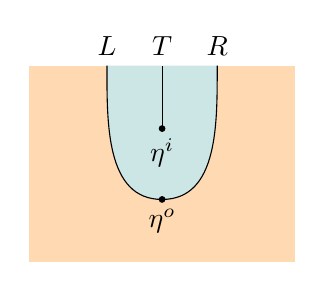
\begin{tikzpicture}
\def\xright{0.7};
\def\xleft{-\xright};
\def\xmid{0};

\def \ybot{0};
\def \ymid{0.8};
\def \yup{1.7};
\def \ytop{2.5};

\node [above] at (\xleft, \ytop) {$L$};
\node [above] at (\xmid, \ytop) {$T$};
\node [above] at (\xright, \ytop) {$R$};

\filldraw[fill=orange!30, draw=white] (\xleft-1, \ytop) rectangle (\xright+1, \ybot);

\draw [fill=blue!50!green!20] (\xleft, \ytop) to [out=-90, in=180] (\xmid, \ymid) to [out=0, in=-90] (\xright, \ytop);

\filldraw[black] (\xmid, \ymid) circle (1 pt);
\node [below] at (\xmid, \ymid) {$\eta^o$};
\filldraw[black] (\xmid, \yup) circle (1 pt);
\node [below] at (\xmid, \yup) {$\eta^i$};
\draw (\xmid, \yup) -- (\xmid,\ytop);

\end{tikzpicture}
\]
It is the vertical composition of the whiskered inner unit $R \circ \eta^i \circ L$ and the outer unit $\eta^o$. In components:
\[ \eta_A = R(\eta^i_{L A}) \circ \eta^o_A\]

The multiplication of the composite monad is a natural transformation:
\[ \mu \colon R \circ T \circ L \circ R \circ T \circ L \to R \circ T \circ L \]
given by the string diagram:

\[
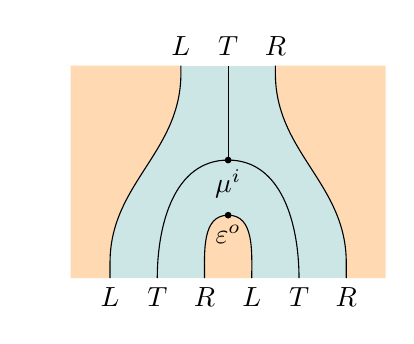
\begin{tikzpicture}
\def \xmid          {0};
\def \xr               {0.3};
\def \xrt             {0.9};
\def \xrr             {1.5}
\def \xrm            {0.6}
\def \xrightmost {2}
\def \xl {-\xr}
\def \xlt {-\xrt}
\def \xll {-\xrr}
\def \xlm {-\xrm}
\def \xleftmost {-\xrightmost}

\def \ybot           {0};
\def \ymidbot     {0.2};
\def \yeps          {0.8};
\def \ymu           {1.5}; % mu
\def \ymid          {1.9};
\def \ymidtop     {2.6}
\def \ytop           {2.7};
\def \ylabel        {\ytop - 0.3};
% functors
\node [above] at (\xlm, \ytop)  {$L$};
\node [above] at (\xmid, \ytop)  {$T$};
\node [above] at (\xrm, \ytop) {$R$};

\node [below] at (\xll, \ybot) {$L$};
\node [below] at (\xlt, \ybot) {$T$};
\node [below] at (\xl, \ybot) {$R$};
\node [below] at (\xr, \ybot) {$L$};
\node [below] at (\xrt, \ybot) {$T$};
\node [below] at (\xrr, \ybot) {$R$};

\filldraw[fill=blue!50!green!20, draw=white, draw=white] (\xleftmost, \ytop) rectangle (\xrightmost, \ybot);

% left area
\path [fill=orange!30] (\xleftmost, \ybot) to  (\xll, \ybot) to (\xll, \ymidbot) [out=90, in=-90] to (\xlm, \ymidtop) to  (\xlm, \ytop) to [out=180, in=180] (\xleftmost, \ytop);
% right area
\path [fill=orange!30] (\xrightmost, \ybot) to (\xrr, \ybot) to (\xrr, \ymidbot) [out=90, in=-90] to (\xrm, \ymidtop) to (\xrm, \ytop) to [out=0, in=180]  (\xrightmost, \ytop);
% cap
\draw [fill=orange!30] (\xl, \ybot) to [out=90, in=180] (\xmid, \yeps) to [out=0, in=90] (\xr, \ybot);
% fork
\draw (\xlt, \ybot) to [out=90, in=180] (\xmid, \ymu) to [out=0, in=90] (\xrt, \ybot);

% left curve
\draw (\xll, \ybot) to (\xll, \ymidbot) [out=90, in=-90] to (\xlm, \ymidtop) to  (\xlm, \ytop);
% right curve
\draw (\xrr, \ybot) to (\xrr, \ymidbot) [out=90, in=-90] to (\xrm, \ymidtop) to (\xrm, \ytop);
% epsilon
\filldraw [black] (\xmid, \yeps) circle (1 pt);
\node [below] at (\xmid, \yeps) {$\varepsilon^o$};

% mu
\filldraw [black] (\xmid, \ymu) circle (1 pt);
\node [below] at (\xmid, \ymu) {$\mu^i$};
\draw (\xmid, \ymu) -- (\xmid, \ytop);

\end{tikzpicture}
\]
It's the vertical composition of the multiply whiskered outer counit:
\[ R \circ T \circ L \circ \varepsilon^o \circ R \circ T \circ L \]
followed by the whiskered inner multiplication $R \circ \mu^i \circ L$. In components:
\[ \mu_C = R(\mu^i_{L C}) \circ (R \circ T) (\varepsilon^o_{(T\circ L)C})\]

Let's unpack these equations for the case of the state monad transformer. Here, the left functor is the product functor \hask{(a, s)} and the right functor is the exponential, a.k.a., the reader functor \hask{s->a}. 

and the counit $\varepsilon^o_Y$ is function application, for the function \hask{f :: x -> y}:
\begin{haskell}
epsilon (f, x) = f x
\end{haskell}
We'll keep the inner monad $(T, \eta^i, \mu^i)$ arbitrary. In Haskell, we'll call these \hask{m}, \hask{return}, and \hask{join}.

The monad that we get by applying the monad transformer for the state monad to the monad $T$, is the composition $R \circ T \circ L$ or, in Haskell:
\begin{haskell}
newtype StateT s m a = StateT (s -> m (a, s))
\end{haskell}

\begin{haskell}
runStateT :: StateT s m a -> s -> m (a, s)
runStateT (StateT h) s = h s
\end{haskell}

The unit of the monad transformer is the composition:
\[ \eta_A = R(\eta^i_{L A}) \circ \eta^o_A \]

There are a lot of moving parts in this formula, so let's analyze it step-by-step. We start from the right: we have the $A$-component of the unit of the adjunction. It's an arrow from $A$ to $R (L A)$. It's tranlated to a Haskell function. If we apply this function to a variable \hask{x :: a}, we can pass the result to the next function in chain, which is $R(\eta^i_{L A})$.

Recall that the unit of the currying adjunction $\eta^o_A$ is defined by:
\begin{haskell}
eta x = \s -> (x, s)
\end{haskell}
so the result is again a function whose type is \hask{s -> (a, s)}. Keep this in mind as we procede. 

Now, what is $R(\eta^i_{LA})$? It's the component of \hask{return} of the inner monad taken at $L A$. Here, $L A$ is the type \hask{(a, s)}. So we are instantiating \hask{return} as a function \hask{(a, s) -> m (a, s)}. (The type inferencer will do this automatically for us.)

Next, we are lifting this component of \hask{return} using $R$. Here, $R$ is the exponential $(-)^S$, so it lifts a function by post-composition. It will post-compose \hask{return} to whatever function is passed to it. That's exactly the function that we produced using \hask{eta}. Notice that the types match: we are post-composing \hask{(a, s) -> m (a, s)} after \hask{s -> (a, s)}. 

We can write the result of this composition as:
\begin{haskell}
return x = StateT (\s -> return (x, s))
\end{haskell}
with the data constructor \hask{StateT} to make the type checker happy. This is the \hask{return} of the composite monad in terms of the \hask{return} of the inner monad.

The same reasoning can be applied to the formula for the component of the composite $\mu$ at some $C$: 
\[ \mu_C = R(\mu^i_{L C}) \circ (R \circ T) (\varepsilon^o_{(T\circ L)C})\]
The inner $\mu^i$ is the \hask{join} of the monad \hask{m}. Applying $R$ turns it into post-composition. 

The outer $\varepsilon^o$ is function application taken at \hask{m (a, s)} which, inserting the appropriate data constructors, can be written as \hask{uncurry runStateT}:
\begin{haskell}
uncurry runStateT :: (StateT s m a, s) -> m (a, s)
\end{haskell}
The application of $(R \circ T)$ lifts this component of $\varepsilon$ using the composition of functors $R$ and $T$. The former is implemented as  post-composition, and the latter is the \hask{fmap} of the monad $m$. 

Putting all this together, we get a point-free formula for \hask{join} of the state monad transformer:
\begin{haskell}
join :: StateT s m (StateT s m a) -> StateT s m a
join mma = StateT (join . fmap (uncurry runStateT) . runStateT mma)
\end{haskell}
Here, the partially applied \hask{runStateT mma} strips off the data constructor from the argument \hask{mma}:
\begin{haskell}
runStateT mma :: s -> m (a, x)
\end{haskell}


identity functor

\section{Monad Algebras}


\section{Monoidal Functors}


\subsection{notes}


\begin{exercise}
\end{exercise}

\begin{haskell}
\end{haskell}

\[
 \begin{tikzcd}
  \end{tikzcd}
\]

\[   \mathbf{Set} \]
\[   \mathcal{C} \]

\end{document}